\chapter{Finitt Element Metode (\glsentrysymbol{fem})}

Den Finite Element Metode (FEM) er en numerisk metode for å løse partielle differensiallikninger.
Metoden går ut på å dele opp domenet i små, enkle geometriske elementer (som trekanter eller firkanter).
Innenfor hvert element tilnærmes løsningen med enkle funksjoner (typisk polynomer).
Til slutt settes elementene sammen for å få en tilnærmet løsning over hele området.


\begin{equation}
  u(x) \approx \sum_{i=1}^N c_i \phi_i(x)
\end{equation}

\section{Teori}

\begin{lemma}{Fundamental lemma of calculus of variations}{fundlemma}
  La $\Omega \subset \mathbb{R}^n$ være et åpent område med regulær rand og $f: \Omega \rightarrow \mathbb{R}$ være en kontinuerlig funksjon. 
  Hvis
  \begin{equation}
    \int_{\Omega} \omega(x) \varphi(x) \, dx = 0 
  \end{equation}
  holder for alle $\varphi \in \Ccal_c^{\infty}(\Omega)$ (dvs. uendelig differensierbare funksjoner med kompakt støtte i $\Omega$), da er $\omega(x) = 0$ for alle $x \in \Omega$.
\end{lemma}

\section{Oversikt}
\begin{enumerate}
  \item Finn \(u: \Omega \rightarrow \R\) slik at \(\Lcal u = f\) i \(\Omega\) og \(u\big|_{\partial\Omega} = g\) på randen \(\partial\Omega\).

  \item Finn \(u \in V := \Hcal_0^1(\Omega)\) slik at \(\inner*{\Lcal u,\Lcal \phi}_\omega = \inner*{f, \phi}_\omega \; \forall \phi \in V\).

  \item Finn \(u_h \in V_h \subset V := \Hcal_0^1(\Omega)\) slik at \(\inner*{\Lcal u_h,\Lcal \phi_i}_\omega = \inner*{f, \phi_i}_\omega \; \forall 1\leq i \leq n\).

  \item Løs \(A\symbf{u} = \symbf{f}\) with \(A_{ij} := \inner*{\Lcal \phi_i, \Lcal \phi_j}\).
\end{enumerate}

\section{\glsentrysymbol{fem}-betingelser}

For å anvende \glsentrysymbol{fem} på en \glsentrysymbol{pde}, må følgende betingelser være oppfylt:

\paragraph{Linearitet} Problemet må kunne uttrykkes i formen \(\Lcal(u) = f\), der \(\Lcal\) er en lineær differensialoperator.

\paragraph{Regularitet} Løsningen \( u(x) \) må ha tilstrekkelig regualritet (kontinuitet og differensierbarhet) innenfor \( \Omega \).
\[
  u \in C^2(\Omega) \quad \text{og} \quad u \in C^1(\partial \Omega)
\]

\paragraph{Diskretisering av domenet} Domenet \( \Omega \) må kunne dekomponeres i ikke-overlappende elementer:
\[
  \Omega = \bigcup_{e=1}^{E} \Omega_e, \quad \Omega_i \cap \Omega_j = \emptyset \text{ for } i \neq j
\]

\paragraph{Approksimativt funksjonsrom} Løsningen må kunne representeres tilfredsstillende ved hjelp av basisfunksjoner:
\[
  u(x) \approx u_h(x) = \sum_{i=1}^{N} c_i \phi_i(x)
\]

\paragraph{Veldefinerte randbetingelser}
Problemet må ha klart definerte randbetingelser:
\begin{itemize}
  \item Dirichlet-betingelser: \( u = g_D \) på \(\partial \Omega_D \)
  \item Neumann-betingelser: \( \nabla u \cdot \mathbf{n} = g_N \) på \(\partial \Omega_N \)
  \item Robin-betingelser: \( \alpha u + \beta \nabla u \cdot \mathbf{n} = g_R \) på \(\partial \Omega_R \)
\end{itemize}

\section{Generell fremgangsmåte}

\begin{enumerate}
  \item \textbf{Definer problemet:} Finn \gls{pde}, over hvilket domene og rand.
        \[
          u: \Omega \to \mathbb{R}, \quad \Lcal(u) = f(x) \quad \text{for } x \in \Omega \quad \text{og} \quad u|_{\partial \Omega} = g
        \]
  \item \textbf{Diskretiser domenet:} Del opp \(\Omega\) i enkle geometriske elementer.
  \item \textbf{Lokal approksimering for hvert element:} Innenfor hvert element (ukjente området/løsning) tilnærmer vi løsningen med en lineærkombinasjon av basisfunksjoner.
        \[
          u(x) \approx \sum_{i=1}^N c_i \phi_i(x)
        \]
  \item \textbf{Fra Sterk til Svak formulering:} Formuler \gls{pde} på \gls{weakformulation}.
        \[
          \int_\Omega v(x) \Lcal(u(x)) \, dx = \int_\Omega v(x) f(x) \, dx
        \]
        \[
          u \in \mathcal{C}^2 \quad \text{s.t.} \quad \Lcal(u) = f \text{ for } x \in \Omega, \; u|_{\partial \Omega} = g
          \implies
          u \in V \quad \text{s.t.} \quad \inner*{\Lcal(u), \Lcal(\phi)} = \inner*{f, \phi} \; \forall \phi \in V
        \]
  \item \textbf{Formuler elementeneligningene:} Sett sammen elementene til et system av ligninger, ved å bruke \gls{weakformulation} av \gls{pde}.
        \[
          \symbf{K} \symbf{u} = \symbf{F}
        \]
  \item \textbf{Randbetingelser:} Sett opp ligningssystemet med randbetingelser.
  \item \textbf{Løs ligningssystemet:} Løs ligningssystemet for å finne koeffisientene \(u_i\).
        \[
          \symbf{u} = \symbf{K}^{-1} \symbf{F}
        \]
\end{enumerate}

\begin{example}{Poisson-ligningen}{poisson}
  \begin{equation}
    \begin{cases}
      -\ddn[2]{u(x)}{x} = f(x),         & x \in (0,1)              \\
      u(0) = \alpha, \quad u(1) = \beta & \text{(randbetingelser)}
    \end{cases}
  \end{equation}

  \begin{equation}
    \mathbf{F} = - \int_0^1 f(x) \mathbf{N}(x) dx
  \end{equation}

  La \(f(x) = \bar{f}\) være konstant. Vi antar at \(u(x_m)\) er ukjent for \(m = 1, \ldots, M\) punkter (noder) i det diskrete domenet \(\Omega_h\).

  I mellom nodene definerer vi \textit{elementene} \(\implies\) \textit{formfunksjoner} \(N_i(x)\).

  \begin{figure}[H]
    \centering
    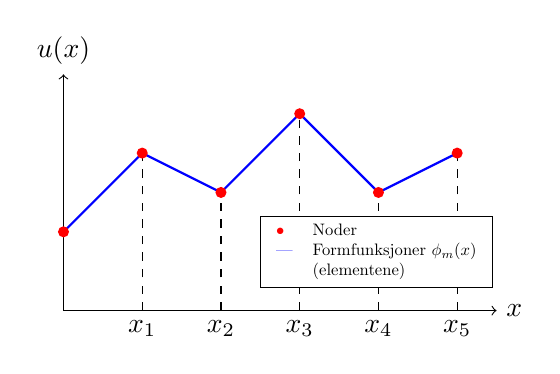
\begin{tikzpicture}
      % Coordinate axes
      \draw[->] (0,0) -- (0,3) node[above] {\(u(x)\)};
      \draw[->] (0,0) -- (5.5,0) node[right] {\(x\)};

      % Solution curve
      \draw[thick, blue] (0,1) -- (1,2) -- (2,1.5) -- (3,2.5) -- (4,1.5) -- (5,2);

      % Vertical lines at nodes with labels
      \draw[dashed] (1,0) node[below] {\(x_1\)} -- (1,2);
      \draw[dashed] (2,0) node[below] {\(x_2\)} -- (2,1.5);
      \draw[dashed] (3,0) node[below] {\(x_3\)} -- (3,2.5);
      \draw[dashed] (4,0) node[below] {\(x_4\)} -- (4,1.5);
      \draw[dashed] (5,0) node[below] {\(x_5\)} -- (5,2);

      % Nodes (intersection points)
      \fill[red] (0,1) circle (2pt);
      \fill[red] (1,2) circle (2pt);
      \fill[red] (2,1.5) circle (2pt);
      \fill[red] (3,2.5) circle (2pt);
      \fill[red] (4,1.5) circle (2pt);
      \fill[red] (5,2) circle (2pt);

      % Add legend
      \node[draw, anchor=north west, scale=0.6,fill=white] at (2.5,1.2) {
        \begin{tabular}{ll}
          \textcolor{red}{\(\bullet\)} & Noder                        \\
          \textcolor{blue}{---}        & Formfunksjoner \(\phi_m(x)\) \\
                                       & (elementene)                 \\
        \end{tabular}
      };
    \end{tikzpicture}
    \caption{Tilfeldig valgt formfunksjoner \(N_i(x)\) mellom nodene \(x_i\).}
  \end{figure}
  Definerer formfunksjonene som:
  \[
    \phi_i(x) = \begin{cases}
      1 - 2|x - x_i|, & |x - x_i| < 0.5 \\
      0,              & \text{ellers}
    \end{cases}
  \]
  Og testfunksjonene som:
  \[
    v(x) = \sum_{j=1}^n v_j \phi_j(x) = \symbf{v}^T \symbf{\phi}(x)
  \]

  Den svake formuleringen blir:
  \begin{align*}
    \int_0^1 \left( \sum_{j=1}^n v_j \phi_j'(x) \right)
    \left( \sum_{i=1}^n u_i \phi_i'(x) \right) \, dx
                        & =
    \int_0^1 \left( \sum_{j=1}^n v_j \phi_j(x) \right) f(x) \, dx \\
    \symbf{v}^T \, \int_0^1 \symbf{\phi}' \symbf{\phi}'^T \, dx \, \symbf{u}
                        & =
    \symbf{v}^T \int_0^1 - f(x) \symbf{\phi}  \, dx               \\
    \symbf{v}^T \symbf{K} \symbf{u}
                        & =
    \symbf{v}^T \symbf{F}                                         \\
    \symbf{K} \symbf{u} & = \symbf{F}
  \end{align*}

  Hvor:

  \begin{align*}
    \symbf{K} & = \int_0^1 \symbf{\phi}' \symbf{\phi}'^T \, dx =
    \begin{bmatrix}
      1  & -1 & 0  & 0  & 0  & 0  \\
      -1 & 2  & -1 & 0  & 0  & 0  \\
      0  & -1 & 2  & -1 & 0  & 0  \\
      0  & 0  & -1 & 2  & -1 & 0  \\
      0  & 0  & 0  & -1 & 2  & -1 \\
      0  & 0  & 0  & 0  & -1 & 1  \\
    \end{bmatrix}                                  \\
    \symbf{F} & = - \bar{f} \int_0^1 \symbf{N}(x) dx
    = - \bar{f}
    \begin{bmatrix}
      0.1 \\ 0.2 \\ 0.2 \\ 0.2 \\ 0.2 \\ 0.1
    \end{bmatrix}
  \end{align*}

  Løser ligningssystemet for å finne koeffisientene \(u_i\):
  \[
    \symbf{u} = \symbf{K}^{-1} \symbf{F}
  \]

\end{example}

\section{Basisfunksjoner (Formfunksjoner)}

Basisfunksjoner er byggesteinene i \gls{fem}-metoden.
De er enkle funksjoner som gjør at vi kan representere en komplisert funksjon ved hjelp av enkle byggesteiner.

En \gls{basisfunction} \(\phi_i(x)\) er en lokal funksjon som:
\begin{itemize}
  \item Er null overalt unntatt i nærheten av node \(i\) (lokalt definert).
  \item Har verdien 1 i node \(i\) og 0 i alle andre noder
  \item Til sammen kan bygge opp løsningen vår \(u(x)\) som en sum:
        \[
          u(x) = \sum_{i=1}^n u_i \phi_i(x) = \symbf{u}^T \symbf{\phi}(x)
        \]
  \item \(u_i\) er koeffisientene som bestemmer hvor mye av hver \gls{basisfunction} som skal brukes.
\end{itemize}


\subsection{Stykkvis lineære basisfunksjoner}

La \(u(x)\) være en tilnærming til løsningen av et \gls{pde}, og la \(u(x)\) være gitt ved en lineærkombinasjon av \gls{basisfunction}er:
\[
  u(x) = \sum_{i=1}^6 u_i N_i(x)
\]


\begin{figure}[H]
  \centering
  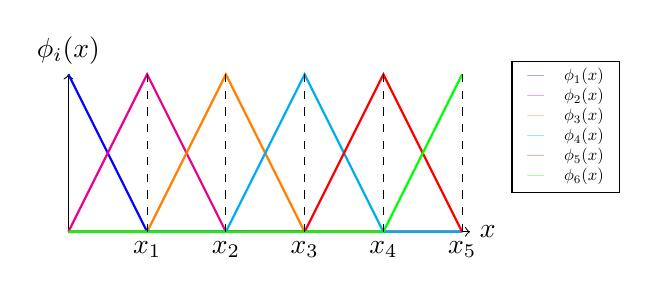
\begin{tikzpicture}
    % Coordinate axes
    \draw[->] (0,0) -- (0,2) node[above] {\(\phi_i(x)\)};
    \draw[->] (0,0) -- (5.1,0) node[right] {\(x\)};

    % Solution curve
    \draw[thick, blue] (0,2) -- (1,0) -- (5,0);
    \draw[thick, magenta] (0,0) -- (1,2) -- (2,0) -- (5,0);
    \draw[thick, orange] (0,0) -- (1,0) -- (2,2) -- (3,0) -- (5,0);
    \draw[thick, cyan] (0,0) -- (2,0) -- (3,2) -- (4,0) -- (5,0);
    \draw[thick, red] (0,0) -- (3,0) -- (4,2) -- (5,0);
    \draw[thick, green] (0,0) -- (4,0) -- (5,2);

    % Vertical lines at nodes with labels
    \draw[dashed] (1,0) node[below] {\(x_1\)} -- (1,2);
    \draw[dashed] (2,0) node[below] {\(x_2\)} -- (2,2);
    \draw[dashed] (3,0) node[below] {\(x_3\)} -- (3,2);
    \draw[dashed] (4,0) node[below] {\(x_4\)} -- (4,2);
    \draw[dashed] (5,0) node[below] {\(x_5\)} -- (5,2);

    % Legend
    \node[draw, anchor=south east, scale=0.6,fill=white] at (7,0.5) {
      \begin{tabular}{ll}
        \textcolor{blue}{---}    & \(\phi_1(x)\) \\
        \textcolor{magenta}{---} & \(\phi_2(x)\) \\
        \textcolor{orange}{---}  & \(\phi_3(x)\) \\
        \textcolor{cyan}{---}    & \(\phi_4(x)\) \\
        \textcolor{red}{---}     & \(\phi_5(x)\) \\
        \textcolor{green}{---}   & \(\phi_6(x)\) \\
      \end{tabular}
    };

  \end{tikzpicture}
  \caption{Piecewise Linear Basis Functions \(\phi_i(x)\)}
\end{figure}

\section{Sterk formulering av \glsentrytext{pde}}
Her skriver vi \glsentrysymbol{pde} direkte i differensialform.
Det betyr at vi forutsetter at løsningen \(u(x)\) er glatt nok til at alle deriverte eksisterer.
Da har vi:
\[
  \Lcal(u) = f,
\]
samt presise krav på grenseverdier, for eksempel:
\[
  u|_{\partial \Omega} = g \quad \text{eller} \quad \frac{\partial u}{\partial n}\bigg|_{\partial \Omega} = h.
\]

Hvis løsningen u ikke er glatt nok, bruker vi en \gls{weakformulation} av problemet.

\section{\glsentrytext{weakformulation} av \glsentrytext{pde}}

Her tester vi u med en \gls{testfunction} \(v(x)\) over hele domenet:
\[
  \int_\Omega v^{(k)}(x) \, \Lcal(u(x)) \, dx = \int_\Omega v(x) \, f(x) \, dx.
\]
Denne metoden gjør det mulig å finne løsninger i et bredere funksjonsrom.

\gls{testfunction} er en vilkårlig funksjon som tilfredsstiller randbetingelsene, og velges ofte til å være det samme som \gls{basisfunction}:
\[
  v(x) = \sum_{j=1}^n v_j \phi_j(x) = \symbf{v}^T \symbf{\phi}(x)
\]

\subsection{\gls{weakformulation} av Poisson-ligningen}
La oss se på Poisson-ligningen:
\[
  -u^{\prime\prime}(x) = f(x), \quad x \in (0,1),
\]
med randbetingelser:
\[
  u(0) = \alpha, \quad u(1) = \beta.
\]
Vi kan skrive den svake formuleringen som:
\[
  \int_0^1 v^\prime (x) u^\prime (x) \, dx = \int_0^1 v(x) f(x) \, dx,
\]
Velger \gls{basisfunction}er til å være:
\[
  \phi_i(x) = \begin{cases}
    1 - 2|x - x_i|, & |x - x_i| < 0.5 \\
    0,              & \text{ellers}
  \end{cases}
\]
Med \gls{testfunction}ene \(v(x) = \sum_{j=1}^n v_j \phi_j(x)\).

Da får vi:

\begin{align*}
  \int_0^1 \left( \sum_{j=1}^n v_j \phi_j'(x) \right)
  \left( \sum_{i=1}^n u_i \phi_i'(x) \right) \, dx
                      & =
  \int_0^1 \left( \sum_{j=1}^n v_j \phi_j(x) \right) f(x) \, dx \\
  \symbf{v}^T \, \int_0^1 \symbf{\phi}' \symbf{\phi}'^T \, dx \, \symbf{u}
                      & =
  \symbf{v}^T \int_0^1 - f(x) \symbf{\phi}  \, dx               \\
  \symbf{v}^T \symbf{K} \symbf{u}
                      & =
  \symbf{v}^T \symbf{F}                                         \\
  \symbf{K} \symbf{u} & = \symbf{F}
\end{align*}


\chapter{\glsentrytext{fem}}

\glsdesc{fem}

\begin{equation}
  u(x) \approx \sum_{i=1}^N c_i \phi_i(x)
\end{equation}

\paragraph{Betingelser}

For å bruke \gls{fem} til å løse et \gls{pde}-problem, må problemet oppfylle følgende betingelser:

\begin{itemize}
  \item \textbf{Linearitet:} Problemet må være lineært, dvs. ligningene kan uttrykkes som \(\Lcal(u) = f\), hvor \(\Lcal\) er en lineær operator.
  \item \textbf{Kontinuerlig Differensierbar:} Løsningen \( u(x) \) må være kontinuerlig differensierbar i \gls{domain}et \( \Omega \).
  \item \textbf{Geometrisk Enkelhet:} \gls{domain}et \( \Omega \) bør kunne deles opp i enkle geometriske elementer (f.eks. trekanter, firkanter i 2D, tetraedre i 3D):
        \[
          \Omega = \bigcup_{e=1}^{E} \Omega_e
        \]
  \item \textbf{Kvantiserbarhet:} Problemet må være kvantiserbart, dvs. løsningen kan tilnærmes godt ved hjelp av en endelig \gls{basisfunction}:
        \[
          u_h(x) = \sum_{i=1}^{N} c_i \phi_i(x)
        \]
  \item \textbf{Randbetingelser:} Randbetingelsene må være kompatible med valg av funksjonsrom:
        \[
          u|_{\partial \Omega} = g \quad \text{eller} \quad \frac{\partial u}{\partial n}\bigg|_{\partial \Omega} = h
        \]
\end{itemize}

\section{Generell fremgangsmåte}

\begin{enumerate}
  \item \textbf{\gls{discretization} 1:} Del \gls{domain} \( \Omega \) inn i enkle geometriske elementer \( \Omega_e \) og tilnærme løsningen med en lineærkombinasjon av \gls{basisfunction}er:
        \[
          u(x) \approx \sum_{i=1}^N c_i \phi_i(x)
        \]
  \item \textbf{\gls{weakformulation}:} Multipliser differensiallikningen med en \gls{testfunction} \( v(x) \) og integrer over \gls{domain}et \( \Omega \):
        \[
          \int_\Omega v(x) \Lcal(u) \, dx = \int_\Omega v(x) f(x) \, dx
        \]

  \item \textbf{Galerkin-prosedyre:} Tilnærme løsningen og \gls{testfunction}en med \gls{basisfunction}er:
        \[
          u(x) \approx \sum_{i=1}^N c_i \phi_i(x) \quad \text{og} \quad v(x) \approx \sum_{j=1}^N d_j \phi_j(x)
        \]
  \item \textbf{\gls{discretization} 2:} Sett inn tilnærmingene i den svake formen og diskretiser:
        \[
          \sum_{j=1}^N d_j \int_\Omega \phi_j(x) \Lcal \left( \sum_{i=1}^N c_i \phi_i(x) \right) \, dx = \sum_{j=1}^N d_j \int_\Omega \phi_j(x) f(x) \, dx
        \]
  \item \textbf{Matriseform:} Skriv den diskretiserte formen som et ligningssett:
        \[
          \symbf{K} \symbf{c} = \symbf{F}
        \]
        Og løs ligningssystemet for å finne koeffisientene \(c_i\):
        \[
          \symbf{c} = \symbf{K}^{-1} \symbf{F}
        \]

\end{enumerate}


\subparagraph{Viktige definisjoner for FEM}
\begin{enumerate}
  \item \textbf{Skalarprodukt} \(\langle v, w \rangle\): Integral av produktet av to funksjoner over \gls{domain}et \(\Omega\):
        \[ \langle v, w \rangle = \int_\Omega v(x)w(x) \, dx \]
        ofte er \(\Omega := (0,1)\).
  \item \textbf{Funksjonsrommet} \(V\): Rommet av funksjoner som tilfredsstiller randbetingelsene.

        \[ V = \{ v \in C^2(\Omega) \, | \, v(a) = \alpha, v(b) = \beta \} \]

  \item \textbf{\gls{testfunction}er} \(v(x)\): Funksjoner i \(V\) som brukes til å formulere den svake formen.
  \item \textbf{\gls{basisfunction}er} \(\phi_i(x)\): Lokale funksjoner som spenner ut løsningsrommet.
        \begin{itemize}
          \item Har kompakt støtte (er null utenfor et lite område)
          \item Oppfyller \(\phi_i(x_j) = \delta_{ij}\) (Kronecker delta)
        \end{itemize}
  \item \textbf{Energifunksjon} \(F(v) = \frac{1}{2} \langle v, v \rangle - \langle f, v \rangle\): Energien til en funksjon \(v\). Kan intuitivt tolkes som en måling av hvor mye energi som kreves for å produsere \(v\).
\end{enumerate}

\subparagraph{FEM for Poisson-ligningen}
\begin{equation}
  \begin{cases}
    -\ddn[2]{u(x)}{x} = f(x),         & x \in (0,1)              \\
    u(0) = \alpha, \quad u(1) = \beta & \text{(randbetingelser)}
  \end{cases}
  \label{eq:pde_poisson}
\end{equation}

\begin{equation}
  \mathbf{F} = - \int_0^1 f(x) \mathbf{N}(x) dx
\end{equation}

La \(f(x) = \bar{f} = C\) være konstant.

Vi antar at \(u(x_m)\) er ukjent for \(m = 1, \ldots, M\) punkter (noder) i det diskrete \gls{domain}et \(\Omega_h\).

I mellom nodene definerer vi \textit{elementene} \(\implies\) \textit{formfunksjoner} \(N_i(x)\).
\begin{figure}[H]
  \centering
  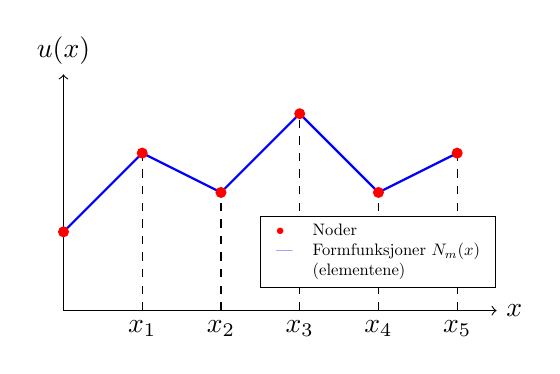
\begin{tikzpicture}
    % Coordinate axes
    \draw[->] (0,0) -- (0,3) node[above] {\(u(x)\)};
    \draw[->] (0,0) -- (5.5,0) node[right] {\(x\)};

    % Solution curve
    \draw[thick, blue] (0,1) -- (1,2) -- (2,1.5) -- (3,2.5) -- (4,1.5) -- (5,2);

    % Vertical lines at nodes with labels
    \draw[dashed] (1,0) node[below] {\(x_1\)} -- (1,2);
    \draw[dashed] (2,0) node[below] {\(x_2\)} -- (2,1.5);
    \draw[dashed] (3,0) node[below] {\(x_3\)} -- (3,2.5);
    \draw[dashed] (4,0) node[below] {\(x_4\)} -- (4,1.5);
    \draw[dashed] (5,0) node[below] {\(x_5\)} -- (5,2);

    % Nodes (intersection points)
    \fill[red] (0,1) circle (2pt);
    \fill[red] (1,2) circle (2pt);
    \fill[red] (2,1.5) circle (2pt);
    \fill[red] (3,2.5) circle (2pt);
    \fill[red] (4,1.5) circle (2pt);
    \fill[red] (5,2) circle (2pt);

    % Add legend
    \node[draw, anchor=north west, scale=0.6,fill=white] at (2.5,1.2) {
      \begin{tabular}{ll}
        \textcolor{red}{\(\bullet\)} & Noder                     \\
        \textcolor{blue}{---}        & Formfunksjoner \(N_m(x)\) \\
                                     & (elementene)              \\
      \end{tabular}
    };
  \end{tikzpicture}
  \caption{Tilfeldig valgt formfunksjoner \(N_i(x)\) mellom nodene \(x_i\).}
\end{figure}

\begin{equation*}
  \symbf{F} = - \bar{f} \int_0^1 \symbf{N}(x) dx = - \bar{f} \begin{bmatrix}
    0.1 \\ 0.2 \\ 0.2 \\ 0.2 \\ 0.2 \\ 0.1
  \end{bmatrix}
\end{equation*}


\section{Basisfunksjoner}

Basisfunksjoner er byggesteinene i \gls{fem}-metoden.
De er enkle funksjoner som gjør at vi kan representere en komplisert funksjon ved hjelp av enkle byggesteiner.

\subparagraph{\gls{basisfunction}}
En \gls{basisfunction} \(\phi_i(x)\) er en lokal funksjon som:
\begin{itemize}
  \item Er null overalt unntatt i nærheten av node \(i\) (lokalt definert).
  \item Har verdien 1 i node \(i\) og 0 i alle andre noder
  \item Til sammen kan bygge opp løsningen vår \(u(x)\) som en sum:
        \[
          u(x) = \sum_{i=1}^n u_i \phi_i(x) = \symbf{u}^T \symbf{\phi}(x)
        \]
  \item \(u_i\) er koeffisientene som bestemmer hvor mye av hver \gls{basisfunction} som skal brukes.
\end{itemize}


\subsection{Stykkvis lineære basisfunksjoner}

La \(u(x)\) være en tilnærming til løsningen av et \gls{pde}, og la \(u(x)\) være gitt ved en lineærkombinasjon av \gls{basisfunction}er:
\[
  u(x) = \sum_{i=1}^6 u_i N_i(x)
\]


\begin{figure}[H]
  \centering
  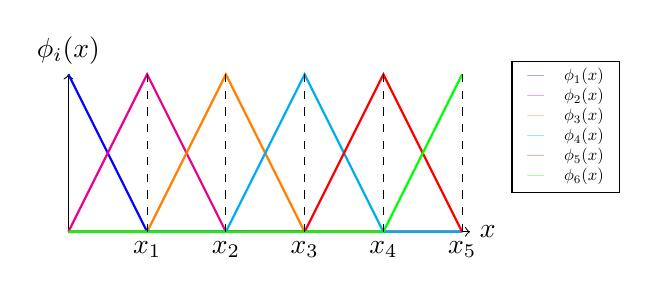
\begin{tikzpicture}
    % Coordinate axes
    \draw[->] (0,0) -- (0,2) node[above] {\(\phi_i(x)\)};
    \draw[->] (0,0) -- (5.1,0) node[right] {\(x\)};

    % Solution curve
    \draw[thick, blue] (0,2) -- (1,0) -- (5,0);
    \draw[thick, magenta] (0,0) -- (1,2) -- (2,0) -- (5,0);
    \draw[thick, orange] (0,0) -- (1,0) -- (2,2) -- (3,0) -- (5,0);
    \draw[thick, cyan] (0,0) -- (2,0) -- (3,2) -- (4,0) -- (5,0);
    \draw[thick, red] (0,0) -- (3,0) -- (4,2) -- (5,0);
    \draw[thick, green] (0,0) -- (4,0) -- (5,2);

    % Vertical lines at nodes with labels
    \draw[dashed] (1,0) node[below] {\(x_1\)} -- (1,2);
    \draw[dashed] (2,0) node[below] {\(x_2\)} -- (2,2);
    \draw[dashed] (3,0) node[below] {\(x_3\)} -- (3,2);
    \draw[dashed] (4,0) node[below] {\(x_4\)} -- (4,2);
    \draw[dashed] (5,0) node[below] {\(x_5\)} -- (5,2);

    % Legend
    \node[draw, anchor=south east, scale=0.6,fill=white] at (7,0.5) {
      \begin{tabular}{ll}
        \textcolor{blue}{---}    & \(\phi_1(x)\) \\
        \textcolor{magenta}{---} & \(\phi_2(x)\) \\
        \textcolor{orange}{---}  & \(\phi_3(x)\) \\
        \textcolor{cyan}{---}    & \(\phi_4(x)\) \\
        \textcolor{red}{---}     & \(\phi_5(x)\) \\
        \textcolor{green}{---}   & \(\phi_6(x)\) \\
      \end{tabular}
    };

  \end{tikzpicture}
  \caption{Piecewise Linear Basis Functions \(\phi_i(x)\)}
\end{figure}

\section{Svak formulering}
\subsection{Fra sterk formulering av PDE}
Her skriver vi \gls{pde}-en direkte i differensialform. Det betyr at vi forutsetter at løsningen u er glatt nok til at alle deriverte eksisterer. Da har vi:
\[
  \Lcal(u) = f,
\]
samt presise krav på grenseverdier, for eksempel:
\[
  u|_{\partial \Omega} = g \quad \text{eller} \quad \frac{\partial u}{\partial n}\bigg|_{\partial \Omega} = h.
\]

\subsection{Til svak formulering av PDE}
For løsninger som ikke er tilstrekkelig glatte, bruker vi en \gls{weakformulation}:

\begin{enumerate}
  \item Multipliser PDE-en med en \gls{testfunction} $v(x)$
  \item Integrer over domenet $\Omega$:
  \[
    \int_\Omega v^{(k)}(x) \, \Lcal(u(x)) \, dx = \int_\Omega v(x) \, f(x) \, dx
  \]
\end{enumerate}

Fordeler: Tillater løsninger i bredere funksjonsrom, reduserer glatthetskrav, og gir mer fleksible randbetingelser.

En \gls{testfunction} $v(x)$ tilfredsstiller randbetingelsene og uttrykkes i Galerkin-metoden ved:
\[
  v(x) = \sum_{j=1}^n v_j \phi_j(x) = \symbf{v}^T \symbf{\phi}(x)
\]


\subparagraph{\gls{weakformulation} av Poisson-ligningen}
La oss se på Poisson-ligningen:
\[
  -u''(x) = f(x), \quad x \in (0,1),
\]
med randbetingelser:
\[
  u(0) = \alpha, \quad u(1) = \beta.
\]
Vi kan skrive den svake formuleringen som:
\[
  \int_0^1 v'(x) u'(x) \, dx = \int_0^1 v(x) f(x) \, dx,
\]
Velger \gls{basisfunction}er til å være:
\[
  \phi_i(x) = \begin{cases}
    1 - 2|x - x_i|, & |x - x_i| < 0.5 \\
    0,              & \text{ellers}
  \end{cases}
\]
Med \gls{testfunction}ene \(v(x) = \sum_{j=1}^n v_j \phi_j(x)\).

Da får vi:

\begin{align*}
  \int_0^1 \left( \sum_{j=1}^n v_j \phi_j'(x) \right) \left( \sum_{i=1}^n u_i \phi_i'(x) \right) \, dx
                      & =
  \int_0^1 \left( \sum_{j=1}^n v_j \phi_j(x) \right) f(x) \, dx \\
  \symbf{v}^T \, \int_0^1 \symbf{\phi}' \symbf{\phi}'^T \, dx \, \symbf{u}
                      & =
  \symbf{v}^T \int_0^1 - f(x) \symbf{\phi}  \, dx               \\
  \symbf{v}^T \symbf{K} \symbf{u}
                      & =
  \symbf{v}^T \symbf{F}                                         \\
  \symbf{K} \symbf{u} & = \symbf{F}
\end{align*}


\section{Sterk formulering}
Gitt $f(x)$, finn $u(x)$ slik at

\begin{align*}
  u^{\prime\prime}(x) & = f(x) \quad \text{for alle } 0 \leq x \leq 1, \\
  u(0)                & = 0,\quad u^{\prime}(1) = 0.
\end{align*}

Introduserer testfunksjonene $v(x)$.
\begin{align*}
  u^{\prime\prime}(x) v(x) & = f(x) v(x)
\end{align*}

Så integrerer vi over intervallet $[0,1]$.
\begin{align*}
  \int_0^1 -u^{\prime\prime}(x) v(x) \, dx & = \int_0^1 f(x) v(x) \, dx
\end{align*}

Alt vi har gjort til nå er å multiplisere med $v(x)$ og integrere over intervallet $[0,1]$, som er generelt lov så lenge $v(x)$ er kontinuerlig og $u(x)$ er to ganger kontinuerlig deriverbar.
Noe den er fra antagelsen om at $u(x)$ er to ganger kontinuerlig deriverbar.

Hvis vi sammenligner integralene på hver side, sier vi egentlig at arealet for $u^{\prime\prime}(x) v(x)$ er lik arealet for $f(x) v(x)$.

\begin{figure}[H]
  \centering
  \begin{minipage}{0.48\textwidth}
    \centering
    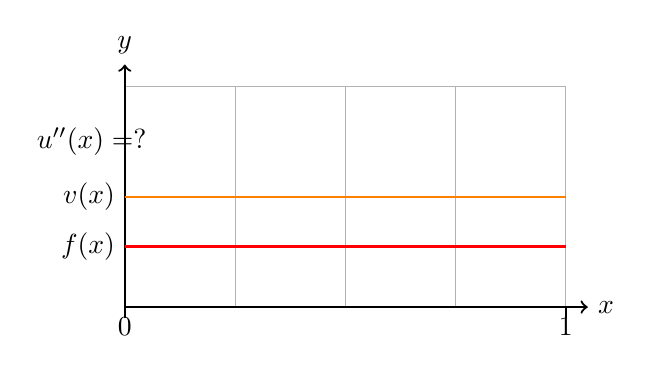
\begin{tikzpicture}[scale=1.4]
      % Grid
      \draw[step=1.0, very thin, black!30] (0,0) grid (4,2);
      \draw[->,thick] (0,0) -- (4.2,0) node[right] {$x$};
      \draw[->,thick] (0,0) -- (0,2.2) node[above] {$y$};
      \draw[thick] (0,-0.1) -- (0,0) node[below] {$0$};
      \draw[thick] (4,-0.1) -- (4,0) node[below] {$1$};

      \draw[orange, thick, domain=0:4, smooth, variable=\x, samples=10] plot (\x, {1});
      \draw[red, thick, domain=0:4, smooth, variable=\x, samples=10] plot (\x, {0.55});

      \node[left] at (0,1) {$v(x)$};
      \node[left] at (0,0.55) {$f(x)$};
      \node[] at (-0.3,1.5) {$u^{\prime\prime}(x) = \displaystyle ?$};
    \end{tikzpicture}
    \caption{Vilkårlig testfunksjon $v(x)$, og kjent $f(x)$}
  \end{minipage}\hfill
  \begin{minipage}{0.48\textwidth}
    \centering
    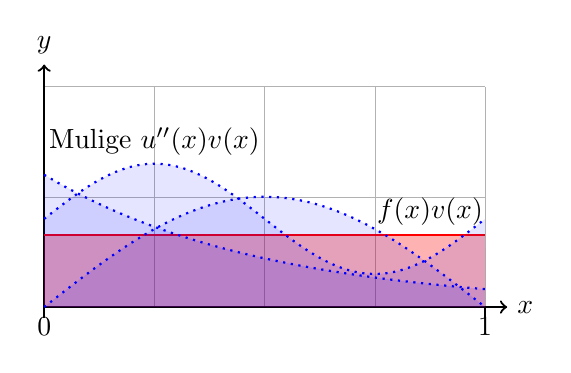
\begin{tikzpicture}[scale=1.4]
      % Grid
      \draw[step=1.0, very thin, black!30] (0,0) grid (4,2);
      \draw[->,thick] (0,0) -- (4.2,0) node[right] {$x$};
      \draw[->,thick] (0,0) -- (0,2.2) node[above] {$y$};
      \draw[thick] (0,-0.1) -- (0,0) node[below] {$0$};
      \draw[thick] (4,-0.1) -- (4,0) node[below] {$1$};

      % Known function f(x)v(x)
      \draw[red, thick, domain=0:4, smooth, variable=\x, samples=100] plot (\x, {0.65});
      \fill[red, opacity=0.3] (0,0) -- plot[domain=0:4, smooth, variable=\x, samples=100] (\x, {0.65}) -- (4,0) -- cycle;

      % Multiple possible u''(x)v(x) functions
      \draw[blue, dotted, thick, domain=0:4, smooth, variable=\x, samples=100] plot (\x, {sin(deg(\x*pi/4))});
      \draw[blue, dotted, thick, domain=0:4, smooth, variable=\x, samples=100] plot (\x, {1.2*exp(-\x/2)});
      \draw[blue, dotted, thick, domain=0:4, smooth, variable=\x, samples=100] plot (\x, {0.8+0.5*sin(deg(\x*pi/2))});

      % Shaded question mark area
      \fill[blue, opacity=0.1] (0,0) -- plot[domain=0:4, smooth, variable=\x, samples=100] (\x, {sin(deg(\x*pi/4))}) -- (4,0) -- cycle;
      \fill[blue, opacity=0.1] (0,0) -- plot[domain=0:4, smooth, variable=\x, samples=100] (\x, {1.2*exp(-\x/2)}) -- (4,0) -- cycle;
      \fill[blue, opacity=0.1] (0,0) -- plot[domain=0:4, smooth, variable=\x, samples=100] (\x, {0.8+0.5*sin(deg(\x*pi/2))}) -- (4,0) -- cycle;

      % Labels
      \node at (1,1.5) {Mulige $u^{\prime\prime}(x) v(x)$};
      \node[above] at (3.5,0.65) {$f(x) v(x)$};
    \end{tikzpicture}
    \caption{Flere mulige løsninger for $u^{\prime\prime}(x)v(x)$, som har samme areal som $f(x)v(x)$}
  \end{minipage}
  \label{ex:svak_formulering}
\end{figure}

I figur \ref{ex:svak_formulering} er det flere mulige løsninger for $u^{\prime\prime}(x)v(x)$, som har samme areal som $f(x)v(x)$.

I dette tilfellet er testfunksjonen vår $v(x) = 1$ forteller ikke dette oss noe mer om hvordan $u^{\prime\prime}(x)$ ser ut.
Altså det gir oss ikke noe mer informasjon om $u^{\prime\prime}(x)$.

Målet vårt nå er å finne/lage en testfunksjon $v(x)$ som faktisk vil kunne gi oss mer informasjon om $u^{\prime\prime}(x)$.

La oss se på testfunksjonen
\[
  v(x) =
  \begin{cases}
    0 & \text{for } x < a,           \\
    1 & \text{for } a \leq x \leq b, \\
    0 & \text{for } b < x.
  \end{cases}
\]
Denne testfunksjonen er lik $1$ bare i intervallet $[a,b]$ og $0$ ellers, som vist i figuren under.


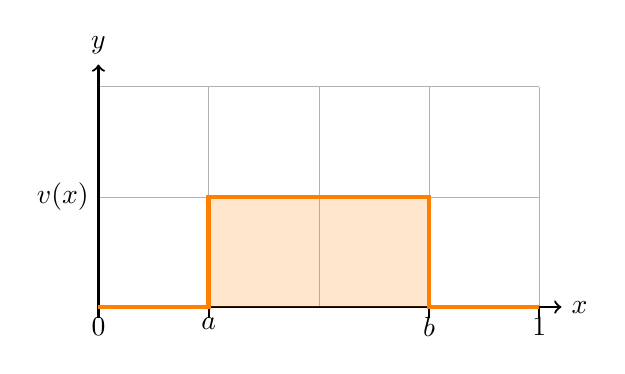
\begin{tikzpicture}[scale=1.4]
  % Grid and axes
  \draw[step=1.0, very thin, black!30] (0,0) grid (4,2);
  \draw[->,thick] (0,0) -- (4.2,0) node[right] {$x$};
  \draw[->,thick] (0,0) -- (0,2.2) node[above] {$y$};
  \draw[thick] (0,-0.1) -- (0,0) node[below] {$0$};
  \draw[thick] (4,-0.1) -- (4,0) node[below] {$1$};

  % Points a and b
  \draw[thick] (1,-0.1) -- (1,0) node[below] {$a$};
  \draw[thick] (3,-0.1) -- (3,0) node[below] {$b$};

  % Test function v(x)
  \draw[orange, ultra thick] (0,0) -- (1,0) -- (1,1) -- (3,1) -- (3,0) -- (4,0);
  \node[left] at (0,1) {$v(x)$};

  % Fill the interval [a,b]
  \fill[orange, opacity=0.2] (1,0) -- (1,1) -- (3,1) -- (3,0) -- cycle;
\end{tikzpicture}

Vi vet at $u^{\prime\prime}(x)$ = f(x) fra den sterke formuleringen. Med vår valgte testfunksjon $v(x)$ får vi:

\begin{align*}
  \int_0^1 u^{\prime\prime}(x) \cdot v(x) \, dx &= \int_0^1 f(x) \cdot v(x) \, dx \\
  \int_0^1 u^{\prime\prime}(x) \cdot v(x) \, dx &= \int_a^b f(x) \cdot 1 \, dx \\
  \int_0^1 u^{\prime\prime}(x) \cdot v(x) \, dx &= \int_a^b f(x) \, dx
\end{align*}

Merk at integralet på høyre side er begrenset til intervallet $[a,b]$ siden $v(x)=0$ utenfor dette intervallet. På samme måte, på venstre side, bidrar $u^{\prime\prime}(x)$ kun til integralet når $x \in [a,b]$.

En nyttig egenskap ved denne tilnærmingen er at hvis vi lar intervallet $[a,b]$ bli veldig lite, slik at $b \rightarrow a$, kan vi intuitivt tenke at:

\begin{align*}
  \int_a^b u^{\prime\prime}(x) \, dx \approx u^{\prime\prime}(a) \cdot (b-a)
\end{align*}

Tilsvarende for høyresiden:

\begin{align*}
  \int_a^b f(x) \, dx \approx f(a) \cdot (b-a)
\end{align*}

Dette gir oss $u^{\prime\prime}(a) \approx f(a)$ når $b \rightarrow a$, som stemmer med vår opprinnelige differensialligning.

\begin{figure}[H]
  \centering
  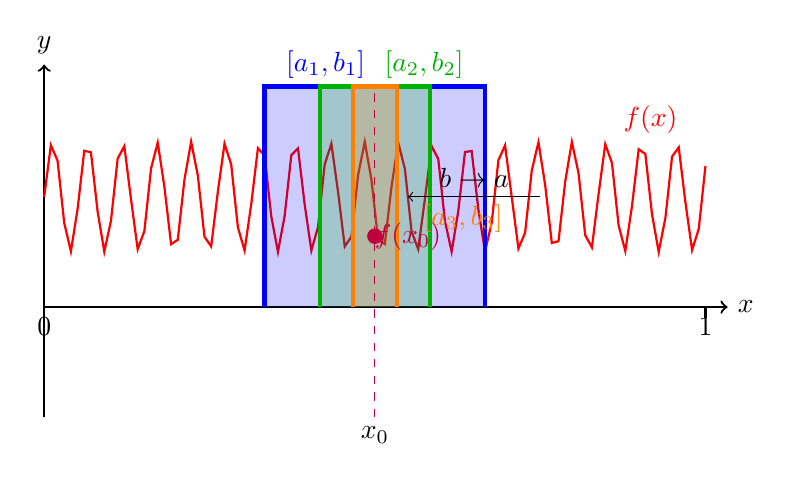
\begin{tikzpicture}[scale=1.4]
    % Axes
    \draw[->,thick] (0,0) -- (6.2,0) node[right] {$x$};
    \draw[->,thick] (0,-1) -- (0,2.2) node[above] {$y$};
    \draw[thick] (0,-0.1) -- (0,0) node[below] {$0$};
    \draw[thick] (6,-0.1) -- (6,0) node[below] {$1$};
    
    % Functions
    \draw[red, thick, domain=0:6, samples=100] plot (\x, {0.5*sin(deg(\x*20))+1});
    \node[red] at (5.5,1.7) {$f(x)$};
    
    % Shrinking intervals
    \draw[blue, ultra thick] (2,0) -- (2,2) -- (4,2) -- (4,0);
    \fill[blue, opacity=0.2] (2,0) -- (2,2) -- (4,2) -- (4,0) -- cycle;
    \node[blue, left] at (3,2.2) {$[a_1,b_1]$};
    
    \draw[green!70!black, ultra thick] (2.5,0) -- (2.5,2) -- (3.5,2) -- (3.5,0);
    \fill[green!70!black, opacity=0.2] (2.5,0) -- (2.5,2) -- (3.5,2) -- (3.5,0) -- cycle;
    \node[green!70!black, right] at (3,2.2) {$[a_2,b_2]$};
    
    \draw[orange, ultra thick] (2.8,0) -- (2.8,2) -- (3.2,2) -- (3.2,0);
    \fill[orange, opacity=0.2] (2.8,0) -- (2.8,2) -- (3.2,2) -- (3.2,0) -- cycle;
    \node[orange] at (3.8,0.8) {$[a_3,b_3]$};
    
    % Point identification at limit
    \draw[purple, dashed] (3,-1) -- (3,2);
    \fill[purple] (3,{0.5*sin(deg(3*50))+1}) circle (2pt);
    \node[purple] at (3.3,{0.5*sin(deg(3*50))+1}) {$f(x_0)$};
    \node[below] at (3,-1) {$x_0$};
    
    \draw[->] (4.5,1) -- (3.3,1) node[midway, above] {$b \rightarrow a$};
  \end{tikzpicture}
  \caption{Når vi gjør intervallet $[a,b]$ stadig mindre, får vi til slutt punktverdien $u^{\prime\prime}(x_0) = f(x_0)$}
  \label{fig:shrinking_interval}
\end{figure}

Men den virkelige styrken med svak formulering kommer når vi bruker delvis integrasjon for å redusere derivasjonsordenene.

\section{Delvis integrasjon og svakere krav til regularitet}

La oss nå anvende delvis integrasjon på den svake formuleringen. Vi har generelt at:

\begin{align*}
  \int_0^1 u^{\prime\prime}(x) v(x) \, dx &= \left. u^{\prime}(x) v(x) \right|_{0}^{1} - \int_0^1 u^{\prime}(x) v^{\prime}(x) \, dx \\
\end{align*}

Med randbetingelsene våre $u(0) = 0$ og $u^{\prime}(1) = 0$, og hvis vi krever at $v(x)$ oppfyller $v(0) = 0$ (siden $u(0) = 0$), får vi:

\begin{align*}
  \int_0^1 u^{\prime\prime}(x) v(x) \, dx &= \left. u^{\prime}(x) v(x) \right|_{0}^{1} - \int_0^1 u^{\prime}(x) v^{\prime}(x) \, dx \\
  &= u^{\prime}(1) v(1) - u^{\prime}(0) v(0) - \int_0^1 u^{\prime}(x) v^{\prime}(x) \, dx \\
  &= 0 \cdot v(1) - u^{\prime}(0) \cdot 0 - \int_0^1 u^{\prime}(x) v^{\prime}(x) \, dx \\
  &= - \int_0^1 u^{\prime}(x) v^{\prime}(x) \, dx
\end{align*}

Dermed blir den svake formuleringen:

\begin{align*}
  \int_0^1 u^{\prime}(x) v^{\prime}(x) \, dx &= \int_0^1 f(x) v(x) \, dx
\end{align*}

Dette er en viktig omformulering fordi:

\begin{enumerate}
  \item Vi trenger nå bare at $u(x)$ er én gang deriverbar, ikke to ganger som i den sterke formuleringen.
  \item Randbetingelsen $u^{\prime}(1) = 0$ er naturlig inkorporert i formuleringen.
  \item Vi kan nå bruke stykkevis lineære funksjoner som har veldefinert første deriverte (nesten overalt), men ikke andre deriverte.
\end{enumerate}

\begin{figure}[H]
  \centering
  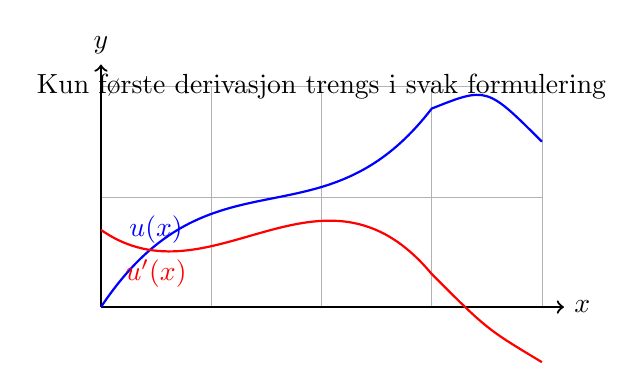
\begin{tikzpicture}[scale=1.4]
    % Grid and axes
    \draw[step=1.0, very thin, black!30] (0,0) grid (4,2);
    \draw[->,thick] (0,0) -- (4.2,0) node[right] {$x$};
    \draw[->,thick] (0,0) -- (0,2.2) node[above] {$y$};
    
    % Original function u(x)
    \draw[blue, thick] (0,0) .. controls (1,1.5) and (2,0.5) .. (3,1.8) .. controls (3.5,2) .. (4,1.5);
    
    % First derivative u'(x)
    \draw[red, thick] (0,0.7) .. controls (1,0) and (2,1.5) .. (3,0.3) .. controls (3.5,-0.2) .. (4,-0.5);
    
    % Labels
    \node[blue] at (0.5,0.7) {$u(x)$};
    \node[red] at (0.5,0.3) {$u'(x)$};
    \node[black] at (2,2) {Kun første derivasjon trengs i svak formulering};
  \end{tikzpicture}
  \caption{I svak formulering trenger vi bare første deriverte av $u(x)$}
  \label{fig:weak_formulation_derivative}
\end{figure}

\section{Sammenligning av sterk og svak formulering}

La oss visualisere forskjellen mellom den sterke og svake formuleringen, samt kravene de stiller til løsningen:

\begin{figure}[H]
  \centering
  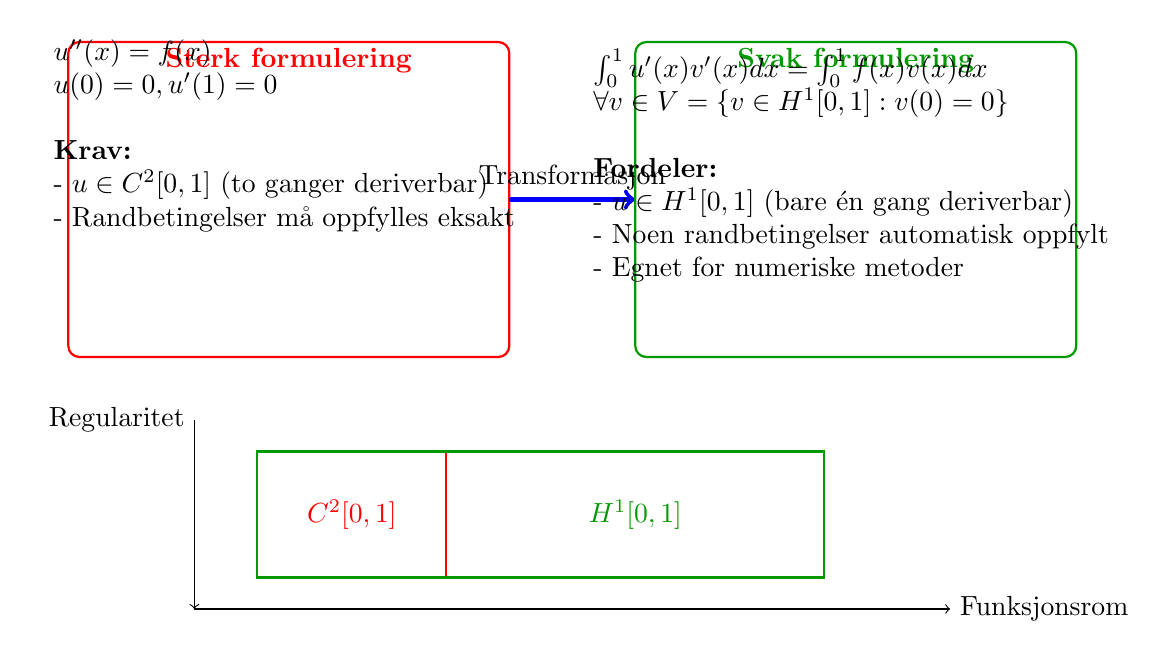
\begin{tikzpicture}[scale=0.8]
    % Box for strong formulation
    \draw[red, thick, rounded corners] (0,0) rectangle (7,5);
    \node[red, font=\bfseries] at (3.5, 4.7) {Sterk formulering};
    
    % Content of strong formulation
    \node[align=left] at (3.5, 3.5) {
      \begin{tabular}{l}
        $u^{\prime\prime}(x) = f(x)$ \\
        $u(0) = 0, u'(1) = 0$ \\
        \\
        \textbf{Krav:} \\
        - $u \in C^2[0,1]$ (to ganger deriverbar) \\
        - Randbetingelser må oppfylles eksakt
      \end{tabular}
    };
    
    \draw[blue, ultra thick, ->] (7,2.5) -- (9,2.5);
    \node[above] at (8,2.5) {Transformasjon};
    
    % Box for weak formulation
    \draw[green!60!black, thick, rounded corners] (9,0) rectangle (16,5);
    \node[green!60!black, font=\bfseries] at (12.5, 4.7) {Svak formulering};
    
    % Content of weak formulation
    \node[align=left] at (12.5, 3) {
      \begin{tabular}{l}
        $\int_0^1 u'(x)v'(x) dx = \int_0^1 f(x)v(x) dx$ \\
        $\forall v \in V = \{v \in H^1[0,1] : v(0) = 0\}$ \\
        \\
        \textbf{Fordeler:} \\
        - $u \in H^1[0,1]$ (bare én gang deriverbar) \\
        - Noen randbetingelser automatisk oppfylt \\
        - Egnet for numeriske metoder
      \end{tabular}
    };
    
    % Function spaces comparison
    \draw[->] (2,-1) -- (2,-4);
    \draw[->] (2,-4) -- (14,-4);
    \node[left] at (2,-1) {Regularitet};
    \node[right] at (14,-4) {Funksjonsrom};
    
    % Function spaces
    \draw[red, thick] (3,-1.5) rectangle (6,-3.5);
    \node[red] at (4.5,-2.5) {$C^2[0,1]$};
    
    \draw[green!60!black, thick] (3,-1.5) rectangle (12,-3.5);
    \node[green!60!black] at (9,-2.5) {$H^1[0,1]$};
  \end{tikzpicture}
  \caption{Sammenligning av sterk og svak formulering av differensialligninger}
  \label{fig:formulation_comparison}
\end{figure}

\section{Sammenheng med endelig element-metoden}

Den svake formuleringen er grunnlaget for endelig element-metoden (FEM). I FEM antar vi at:

\begin{align*}
  u(x) &\approx \sum_{i=1}^n c_i \varphi_i(x) \\
  v(x) &= \varphi_j(x) \quad \text{for } j=1,2,...,n
\end{align*}

hvor $\varphi_i(x)$ er basisfunksjoner (typisk stykkevis lineære funksjoner). Ved å sette disse uttrykkene inn i den svake formuleringen, får vi et lineært ligningssystem for koeffisientene $c_i$:

\begin{align*}
  \sum_{i=1}^n c_i \int_0^1 \varphi_i^{\prime}(x) \varphi_j^{\prime}(x) \, dx &= \int_0^1 f(x) \varphi_j(x) \, dx \quad \text{for } j=1,2,...,n
\end{align*}

Dette kan skrives på matriseform som:

\begin{align*}
  \mathbf{K} \mathbf{c} = \mathbf{F}
\end{align*}

hvor:
\begin{align*}
  K_{ji} &= \int_0^1 \varphi_i^{\prime}(x) \varphi_j^{\prime}(x) \, dx \\
  F_j &= \int_0^1 f(x) \varphi_j(x) \, dx
\end{align*}

Denne formuleringen er grunnlaget for numerisk løsning av differensialligninger ved hjelp av endelig element-metoden.

\begin{figure}[H]
  \centering
  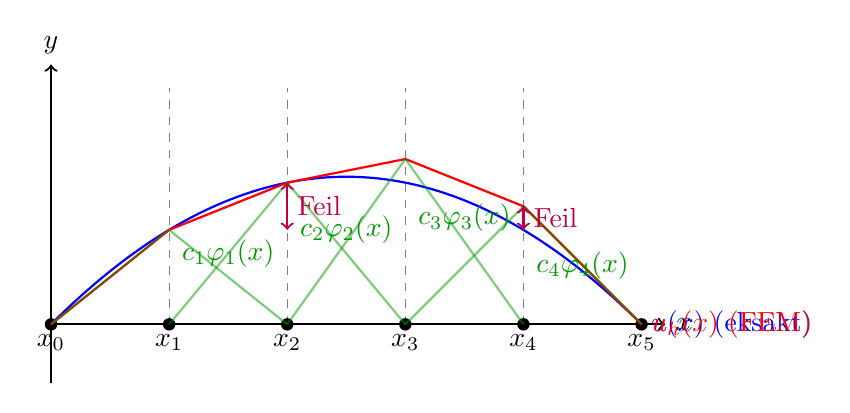
\begin{tikzpicture}[scale=1.5]
    % Axes
    \draw[->,thick] (0,0) -- (5.2,0) node[right] {$x$};
    \draw[->,thick] (0,-0.5) -- (0,2.2) node[above] {$y$};
    
    % Grid
    \foreach \x in {1,2,3,4}
      \draw[dashed,gray] (\x,0) -- (\x,2);
    
    % Node points
    \foreach \x in {0,1,2,3,4,5}
      \fill (\x,0) circle (1.5pt) node[below] {$x_{\x}$};
    
    % True solution
    \draw[thick, blue, domain=0:5, samples=100] 
      plot (\x, {0.2*\x*(5-\x)});
    \node[blue, right] at (5, 0) {$u(x)$ (eksakt)};
    
    % FEM solution
    \draw[thick, red] (0,0) -- (1,0.8) -- (2,1.2) -- (3,1.4) -- (4,1.0) -- (5,0);
    \node[red, right] at (5, 0) {$u_h(x)$ (FEM)};
    
    % Basis functions - scaled by coefficients
    \draw[green!60!black, thick, opacity=0.5] (0,0) -- (1,0.8) -- (2,0);
    \draw[green!60!black, thick, opacity=0.5] (1,0) -- (2,1.2) -- (3,0);
    \draw[green!60!black, thick, opacity=0.5] (2,0) -- (3,1.4) -- (4,0);
    \draw[green!60!black, thick, opacity=0.5] (3,0) -- (4,1.0) -- (5,0);
    
    \node[green!60!black] at (1.5, 0.6) {$c_1\varphi_1(x)$};
    \node[green!60!black] at (2.5, 0.8) {$c_2\varphi_2(x)$};
    \node[green!60!black] at (3.5, 0.9) {$c_3\varphi_3(x)$};
    \node[green!60!black] at (4.5, 0.5) {$c_4\varphi_4(x)$};
    
    % Error indication
    \draw[<->,purple,thick] (2,1.2) -- (2,0.8) node[midway,right] {Feil};
    \draw[<->,purple,thick] (4,1.0) -- (4,0.8) node[midway,right] {Feil};
  \end{tikzpicture}
  \caption{FEM-løsning ($u_h(x)$) som en sum av vektede basisfunksjoner, sammenlignet med den eksakte løsningen ($u(x)$)}
  \label{fig:fem_solution}
\end{figure}

\begin{figure}[H]
  \centering
  \begin{tikzpicture}[scale=1.5, transform shape]
    % Axes
    \draw[->,thick] (0,0) -- (2.2,0) node[right] {$x$};
    \draw[->,thick] (0,0) -- (0,1.2) node[above] {$y$};
    
    % Mesh points
    \foreach \x in {0,0.5,1,1.5,2}
      \fill (\x,0) circle (0.5pt) node[below=1pt] {$\x$};
    
    % System matrix visualization
    \matrix [matrix of nodes, nodes={minimum size=6mm}, 
             row sep=-\pgflinewidth, column sep=-\pgflinewidth,
             draw=black, thick, outer sep=0pt,
             anchor=north west] (K) at (2.5,1) {
      |[fill=red!20]| $2$ & |[fill=red!15]| $-1$ & |[fill=red!5]| $0$ & |[fill=red!5]| $0$ \\
      |[fill=red!15]| $-1$ & |[fill=red!20]| $2$ & |[fill=red!15]| $-1$ & |[fill=red!5]| $0$ \\
      |[fill=red!5]| $0$ & |[fill=red!15]| $-1$ & |[fill=red!20]| $2$ & |[fill=red!15]| $-1$ \\
      |[fill=red!5]| $0$ & |[fill=red!5]| $0$ & |[fill=red!15]| $-1$ & |[fill=red!20]| $2$ \\
    };
    \node[above=1mm] at (K.north) {$\mathbf{K}$ (stivhetsmatrise)};
    
    % Solution vector
    \matrix [matrix of nodes, nodes={minimum size=6mm}, 
             row sep=-\pgflinewidth, column sep=-\pgflinewidth,
             draw=black, thick, outer sep=0pt,
             anchor=north west] (u) at (4.0,1) {
      |[fill=blue!20]| $c_1$ \\
      |[fill=blue!20]| $c_2$ \\
      |[fill=blue!20]| $c_3$ \\
      |[fill=blue!20]| $c_4$ \\
    };
    \node[above=1mm] at (u.north) {$\mathbf{c}$};
    
    % Equals sign
    \node at (4.5,0.45) {$=$};
    
    % Right-hand side vector
    \matrix [matrix of nodes, nodes={minimum size=6mm}, 
             row sep=-\pgflinewidth, column sep=-\pgflinewidth,
             draw=black, thick, outer sep=0pt,
             anchor=north west] (f) at (5.0,1) {
      |[fill=green!15]| $F_1$ \\
      |[fill=green!15]| $F_2$ \\
      |[fill=green!15]| $F_3$ \\
      |[fill=green!15]| $F_4$ \\
    };
    \node[above=1mm] at (f.north) {$\mathbf{F}$};
    
    % Example basis functions
    \draw[thick, blue] (0,0) -- (0.5,1) -- (1,0);
    \draw[thick, red] (0.5,0) -- (1,1) -- (1.5,0);
    \draw[thick, green!60!black] (1,0) -- (1.5,1) -- (2,0);
    
    % Labels
    \node[blue, scale=0.8] at (0.4,0.6) {$\varphi_1(x)$};
    \node[red, scale=0.8] at (0.9,0.6) {$\varphi_2(x)$};
    \node[green!60!black, scale=0.8] at (1.5,0.6) {$\varphi_3(x)$};
  \end{tikzpicture}
  \caption{FEM diskretisering: basisfunksjoner $\varphi_i(x)$ og tilhørende ligningssystem $\mathbf{K}\mathbf{c} = \mathbf{F}$}
  \label{fig:fem_discretization}
\end{figure}